\documentclass[11pt]{ctexart}
% \documentclass{article}
\textheight 23.5cm \textwidth 15.8cm
%\leftskip -1cm
\topmargin -1.5cm \oddsidemargin 0.3cm \evensidemargin -0.3cm

\usepackage{verbatim}
\usepackage{fancyhdr}
\usepackage{graphicx}
\usepackage{amssymb}
\usepackage{amsmath}
\usepackage{subcaption}
\ctexset {
     section/format    += \sffamily\raggedright,
     subsection/format += \fbox,
}


\title{FEM Code Report 1}
\author{SA24229016 王润泽}

\begin{document}
\maketitle

\section{Introduction}
	编写程序求解以下两点边值问题:
	\begin{equation}
		\begin{aligned}
			-u'' &= f, \quad 0 < x < 1, \\
			u(0) &= u(1) = 0.
		\end{aligned}
	\end{equation}
	其中取 $ f(x) = -(2\cos{x}-(x-1)\sin{x}) $,已知其解析解为 $ u(x) = (x-1)\sin{x} $。
\section{Method}

	给定双线性形式 $a(u,v)$ 和内积 $(f, g)$,定义如下:
	\begin{equation}
		a(u,v) = \int_0^1 u' v' \, dx,
		\label{eq:double_linear}
	\end{equation}
	\begin{equation}
		(f, g) = \int_0^1 f \cdot g \, dx.
		\label{eq:inner_product}
	\end{equation}

	由此,问题 (1) 的变分形式为:  
	寻找 $u \in \mathcal{V} = \{v \in C[0,1], v(0) = v(1) = 0\}$,使得对所有 $v \in \mathcal{V} $,均有:
	\begin{equation}
		a(u,v) = (f,v).
	\end{equation}

	实验中采用等距网格划分,节点数为 $N+1$,在每个节点处的函数值记为 $u_i$,网格步长为 $h = 1/N$。选取基函数 $\varphi_i$,并通过这些基函数所张成的有限维线性空间进行求解。此时得到原问题的离散形式解为:$ u_h = \sum_{i=1}^{N} u_i \varphi_i $,其中 $u_i$ 为待求解的系数, 而 $ v_h = \sum_{i=1}^{N} v_i \varphi_i $。 
	
	基函数定义如下:
	\begin{equation}
		\varphi_i(x) = 
		\begin{cases} 
		\frac{x - x_{i-1}}{x_i - x_{i-1}}, & x \in [x_{i-1}, x_i), \\
		\frac{x_{i+1} - x}{x_{i+1} - x_i}, & x \in [x_i, x_{i+1}], \\
		0, & \text{otherwise}.
		\end{cases}
	\end{equation}

	
	
	对于公式 \eqref{eq:double_linear}离散化得到:
	\begin{equation}
		a(\varphi_i, \varphi_j)=\left\{
		\begin{aligned}
			&-\frac{1}{h}, & |i-j| = 1\\
			&\frac{2}{h}, &i = j\\
			&0,  &\text{otherwise}
		\end{aligned}
		\right.
	\end{equation}
	
	因此,刚度矩阵为:
	\begin{equation}
		A = \frac{1}{h}\begin{bmatrix}
			2 & -1 & 0 & \cdots & 0 \\
			-1 & 2 & -1 & \cdots & 0 \\
			0 & -1 & 2 & \cdots & 0 \\
			\vdots & \vdots & \vdots & \ddots & \vdots \\
			0 & 0 & 0 & \cdots & 2
		\end{bmatrix}
	\end{equation}

	根据公式 \eqref{eq:inner_product},得到对各个基函数与 $f$ 的内积,即荷载向量各项为:
	\begin{equation}
		f_i = (f, \varphi_i) = \int_0^1 f \varphi_i \, dx = 4(hj-1)\sin^2(h/2)sin(hj)/h-2\sin(h)\cos(hj)
	\end{equation}

	以上,得到变分问题的离散形式为,对任意的 $ V=(v_1,v_2,\cdots,v_{N})^T $,有: 
	\begin{equation}
		V^TAU = V^TF
	\end{equation}

	进一步,只要求解出 $ AU = F $ 即可得到 $ U $,即为问题 (1) 的数值解,其中:
	\begin{equation}
		\begin{aligned}
			U &= (u_1, u_2, \cdots, u_{N})^T, \\
			F &= (f_1, f_2, \cdots, f_{N})^T.
		\end{aligned}
	\end{equation} 

\section{Results}

\subsection{数值拟合效果}
通过调整 $N=\{10,20,40,80\}$ 的值,得到不同的数值解,与解析解进行比较,如图 \ref{fig:fit} 所示。

\begin{figure}[htbp]
    \centering
    \begin{subfigure}{0.45\textwidth}
        \centering
        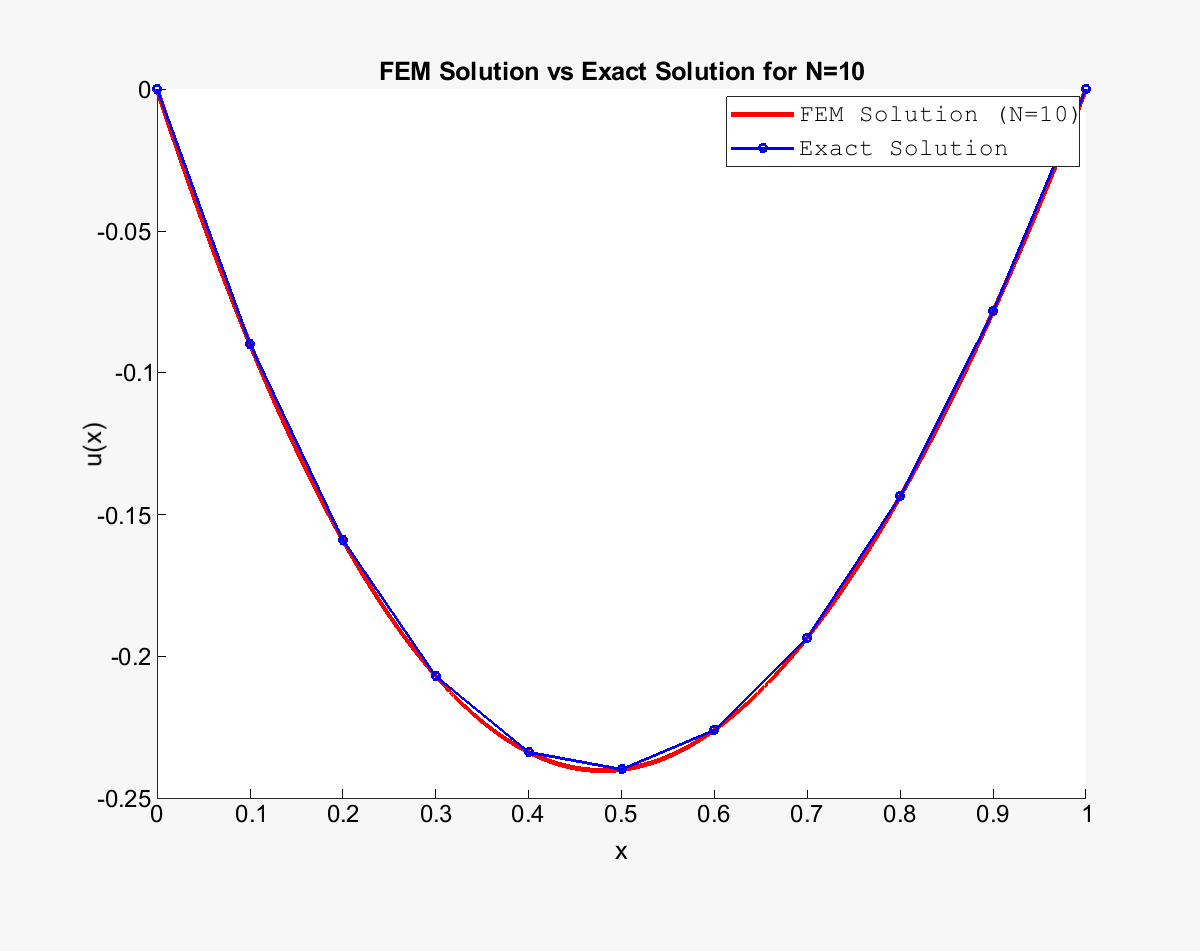
\includegraphics[width=\linewidth]{10.png}
        \caption{$ N=10 $ }
        \label{fig:sub1}
    \end{subfigure}
    \hfill
    \begin{subfigure}{0.45\textwidth}
        \centering
        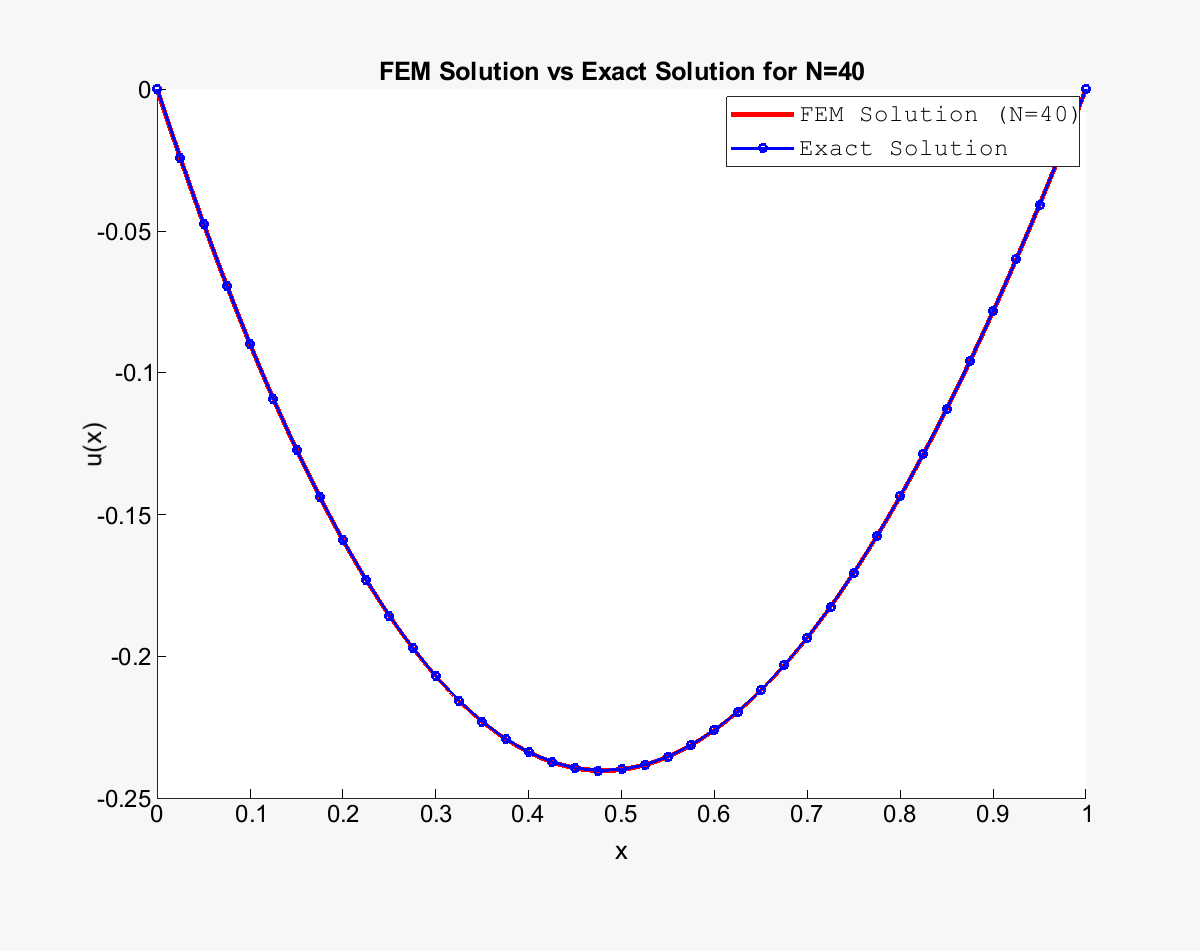
\includegraphics[width=\linewidth]{40.png}
        \caption{$ N=40 $ }
        \label{fig:sub2}
    \end{subfigure}
    
    % 第二行的两张图
    \vspace{1em}
    
    \begin{subfigure}{0.45\textwidth}
        \centering
        \includegraphics[width=\linewidth]{image3.png}
        \caption{图 3}
        \label{fig:sub3}
    \end{subfigure}
    \hfill
    \begin{subfigure}{0.45\textwidth}
        \centering
        \includegraphics[width=\linewidth]{image4.png}
        \caption{图 4}
        \label{fig:sub4}
    \end{subfigure}
    
    \caption{四个子图的排列示例}
    \label{fig:four_figs}
\end{figure}

\subsection{误差分析}
已知其解析解为:
\begin{equation}
    u(x) = (x - 1) \sin x.
\end{equation}
完成数值求解后,使用 $L^2$ 范数和 $H^1$ 范数计算误差,并对结果进行讨论。$L^2$ 范数的定义为:
\begin{equation}
    \| e \|_{L^2} = \left( \int_0^1 (u(x) - u_h(x))^2 \, dx \right)^{1/2},
\end{equation}
$H^1$ 范数的定义为:
\begin{equation}
    \| e \|_{H^1} = \left( \int_0^1 \left( (u(x) - u_h(x))^2 + (u'(x) - u_h'(x))^2 \right) dx \right)^{1/2}.
\end{equation}

\section{Discussion}


\appendix
\section{Computer Code}

\end{document}